%\appendix
%\chapter{1}

\begin{appendices}
%\chapter{Simulator}
\chapter{PathBench} \label{sec: app_env}

\section{Infrastructure} \label{sec: infra}
The \textbf{MainRunner} component is the main entry point of the platform and it coordinates all other sections. The \textbf{MainRunner} takes a master \textbf{Configuration} component as input which represents the main inflexion point of the platform. It describes which section (\textbf{Simulator}, \textbf{Generator}, \textbf{Trainer}, \textbf{Analyser}) should be used and how (The master \textbf{Configuration} fields can be seen in Tables \ref{tab: sim_master_config}, \ref{tab: generator_master_config} and \ref{tab: trainer_master_config}).

The \textbf{Services} component is a bag of \textbf{Service} components which is injected into all platform classes in order to maintain global access to the core libraries\footnote{Design known as Dependency Injection or Strategy Pattern \cite{hannemann2002design}}. A \textbf{Service} component is created for most external libraries to encapsulate their APIs and provide useful helper functions\footnote{Design known as the Adapter Pattern \cite{hannemann2002design}}. Moreover, by making use of the Adapter Pattern we can easily switch third party libraries, if needed, and the code becomes more test friendly. Finnaly, the \textbf{Services} container can be mocked together with all its \textbf{Service} components, thus avoiding rendering, file writing and useless printing.

The \textbf{Simulator} was build by following the Model-View-Controller (MVC) pattern \cite{krasner1988description}. The \textbf{Model} represents the logic part, the \textbf{View} renders the \textbf{Model} and the \textbf{Controller} handles the input from the keyboard and mouse, and calls the appropriate functions from the associated \textbf{Model}. The \textbf{EventManager} component is a communication service which allows the \textbf{Model} to update the \textbf{View} as there is no direct connection between them (from \textbf{Model} to \textbf{View}, the other way is).

The \textbf{Debug} component is a printing service which augments printing messages with different decorators such as time-stamp and routes the messages to a specified IO stream or standard out. It also provides a range of debugging/printing modes: None (no information), Basic (only basic information), Low (somewhat verbose), Medium (quite verbose), High (all information).

The \textbf{RenderingEngine} component is a wrapper around the \textit{pygame} library and all rendering is routed through it.

The \textbf{Torch} service is not an actual wrapper around \textit{pytorch}, but instead it defines some constants such as the initial random seed and the training device (CPU/CUDA).

The \textbf{Resources} service is the persistent storage system. It is a container of \textbf{Directory} components which represent an interface over the actual filesystem directories. It provides safe interaction with the filesystem and a range of utility directories: Cache (temporary storage used for speeding second runs), Screenshots, Maps (stores all user defined and generated maps), Images (stores images which can be converted to internal maps), Algorithms (stores trained machine learning models), Training Data (stores training data for machine learning models). The main serialisation tool is \textit{dill} which is a wrapper around \textit{pickle} with lambda serialisation capabilities, but custom serialisation is allowed such as tensor serialisation provided by \textit{pytorch} or image saving by \textit{pygame}.

The \textbf{AlgorithmRunner} manages the algorithm session which contains the \textbf{Algorithm}, \textbf{BasicTesting} and \textbf{Map}. The \textbf{AlgorithmRunner} launches a separate daemon thread that is controlled by a condition variable. When writing an \textbf{Algorithm}, special key frames can be defined (e.g. when the trace is produced) to create animations. Key frames release the synchronisation variable for a brief period and then acquire it again, thus querying new rendering jobs.

The \textbf{Utilities} section provides a series of helper methods and classes: \textbf{Maps} (holds in-memory user defined \textbf{Map} components), \textbf{Point}, \textbf{Size}, \textbf{Progress} (progress bar), \textbf{Timer}, \textbf{MapProcessing} (feature extractor used mainly in ML sections).

\section{Master Configuration and User Commands}

\begin{table}[h!]
    \footnotesize
    \centerfloat
    \begin{tabular}{|c|M{2.45cm}|M{7cm}|}
        \hline
        \textbf{Configuration Field} & \textbf{Type} & \textbf{Description} \\
        \hline
        load\_simulator & \texttt{bool} & If the simulator should be loaded \\
        \hline
        clear\_cache & \texttt{bool} & If the cache should be deleted after the simulator is finished \\
        \hline
        simulator\_graphics & \texttt{bool} & If graphics should be used or not; evaluation is always done without graphics \\
        \hline
        simulator\_grid\_display & \texttt{bool} & The map can be visualised as a plain image or a grid; the window size is defined based on the choice \\
        \hline
        simulator\_initial\_map & \texttt{Map} & The map used in \textbf{AlgorithmRunner} service\\
        \hline
        simulator\_algorithm\_type & \texttt{Type[Algorithm]} & The algorithm type used in \textbf{AlgorithmRunner} service\\
        \hline
        simulator\_algorithm\_parameters & \texttt{Tuple[List[Any], Dict[str, Any]]} & The algorithm parametrs in the form of *args and **kwargs which are used in  \textbf{AlgorithmRunner} service\\
        \hline
        simulator\_testing\_type & \texttt{Type[BasicTesting]} & The testing type used in \textbf{AlgorithmRunner} service\\
        \hline
        simulator\_key\_frame\_speed & \texttt{int} & The refresh rate interval during each key frame; a value of 0 disables the key frames \\
        \hline
        simulator\_key\_frame\_skip & \texttt{int} & How many key frames are skipped at a time; used to speed up the animation when frames per second are low \\
        \hline
        simulator\_write\_debug\_level & \texttt{DebugLevel} & The debugging level (None, Basic, Low, Medium, High) \\
        \hline
    \end{tabular}
    \caption{Simulator master \textbf{Configuration} fields}
    \label{tab: sim_master_config}
\end{table}

\pagebreak

\begin{table}[h!]
    \footnotesize
    \centerfloat
    \begin{tabular}{|c|M{2cm}|M{6cm}|}
        \hline
        \textbf{Configuration Field} & \textbf{Type} & \textbf{Description} \\
        \hline
        generator & \texttt{bool} & If the generator should be loaded \\
        \hline
        generator\_gen\_type & \texttt{str} & Generation type; can choose between "uniform\_random\_fill", "block\_map" and "house" (See Figure \ref{fig: generated maps}) \\
        \hline
        generator\_nr\_of\_examples & \texttt{int} & How many maps should be generated; 0 does not trigger generation \\
        \hline
        generator\_labelling\_atlases & \texttt{List[str]} & Which \textbf{Map Atlas}es should be converted to training data\\
        \hline
        generator\_labelling\_features & \texttt{List[str]} & Which sequential features should be extracted for training conversion \\
        \hline
        generator\_labelling\_labels & \texttt{List[str]} & Which sequential labels should be extracted for training conversion \\
        \hline
        generator\_single\_labelling\_features & \texttt{List[str]} & Which single features should be extracted for training conversion \\
        \hline
        generator\_single\_labelling\_labels & \texttt{List[str]} & Which single labels should be extracted for training conversion \\
        \hline
        generator\_aug\_labelling\_features & \texttt{List[str]} & Which sequential features should be augmented for training data defined by generator\_labelling\_atlases \\
        \hline
        generator\_aug\_labelling\_labels & \texttt{List[str]} & Which sequential labels should be augmented for training data defined by generator\_labelling\_atlases \\
        \hline
        generator\_aug\_single\_labelling\_features & \texttt{List[str]} & Which single features should be augmented for training data defined by generator\_labelling\_atlases \\
        \hline
        generator\_aug\_single\_labelling\_labels & \texttt{List[str]} & Which single labels should be augmented for training data defined by generator\_labelling\_atlases \\
        \hline
        generator\_modify & \texttt{Callable[[Map], Map]} & Modifies the given map using the custom function \\
        \hline
    \end{tabular}
    \caption{Generator master \textbf{Configuration} fields}
    \label{tab: generator_master_config}
\end{table}

\begin{table}[h!]
    \footnotesize
    \centerfloat
    \begin{tabular}{|c|M{2.2cm}|M{4.5cm}|}
        \hline
        \textbf{Configuration Field} & \textbf{Type} & \textbf{Description} \\
        \hline
        trainer & \texttt{bool} & If the trainer should be loaded \\
        \hline
        trainer\_model & \texttt{Type[MLModel]} & The model which will be trained \\
        \hline
        trainer\_custom\_config & \texttt{Dict[str, Any]} & If a custom configuration should augment the \textbf{MLModel} configuration \\
        \hline
        trainer\_pre\_process\_data\_only & \texttt{bool} & If the trainer should only pre-process data and save it; it does not overwrite cache\\
        \hline
        trainer\_bypass\_and\_replace\_pre\_processed\_cache & \texttt{bool} & If pre-processed data cache should be bypassed and re-computed \\
        \hline
    \end{tabular}
    \caption{Trainer master \textbf{Configuration} fields}
    \label{tab: trainer_master_config}
\end{table}

\begin{table}[h!]
    \centerfloat
    \begin{tabular}{|c|c|}
        \hline
        \textbf{Key} & \textbf{Action} \\
        \hline
        up arrow & moves agent up \\
        \hline
        left arrow & moves agent left \\
        \hline
        down arrow & moves agent down \\
        \hline
        right arrow & moves agent right \\
        \hline
        c & compute trace \\
        \hline
        s & stop trace animation (requires key frames) \\
        \hline
        r & resume trace animation (requires key frames) \\
        \hline
        m & toggle map between \textbf{SparseMap} and \textbf{DenseMap} \\
        \hline
        p & take map screenshot \\
        \hline
        mouse hover & reports hovered cell coordinates (requires at least Medium debugging level) \\
        \hline
        mouse left click & moves \textbf{Agent} to mouse location \\
        \hline
        mouse right click & moves \textbf{Goal} to mouse location \\
        \hline
    \end{tabular}
    \caption{Simulator user commands}
    \label{tab: sim_commands}
\end{table}



\chapter{Methods} \label{sec: app_methods}

\section{Packing and Unpacking}

Packing is used to speed up the forward pass through the LSTM layer and mask unused data (because data is given as a variable length sequence). By making use of packing, we can remove the need to pad the inputs with a special token in order to convert the variable size sequence into a constant size sequence. Moreover, if the pad token is not chosen correctly the network might learn from it and become biased towards one action (e.g. if the labelling pad token is 0, then the 0 action might get preferred over the other actions). When packing a batch sequence, all sequences have to be sorted in reverse order of the sequence length (largest sequence first). The packing is done by using the function \texttt{pack\_sequence} from \textit{pytorch} which returns a \texttt{PackedSequence} object. The \texttt{PackedSequence} transforms the data into a continuous 1D tensor by concatenating all batch tensors. The structure of the original data is still preserved into the \texttt{batch\_sizes} attribute. The whole packing procedure has complexity $\mathcal{O}(n\log(n))$ (sorting is $\mathcal{O}(n\log(n))$ and \texttt{pack\_sequence} is $\mathcal{O}(n)$, where $n$ is the batch size). The following code snippet showcases an example of the packing procedure:

\begin{lstlisting}[language=Python]
import torch
from torch.nn.utils.rnn import pack_sequence, PackedSequence

a = torch.Tensor([1, 2])
b = torch.Tensor([3, 4, 5])
c = torch.Tensor([6])
seq = [a, b, c]
seq.sort(key=lambda el: el.shape[0], reverse=True)
packed_sequence: PackedSequence = pack_sequence(seq)

# Output: PackedSequence(data=tensor([3., 1., 6., 4., 2., 5.]), 
#                        batch_sizes=tensor([3, 2, 1]))
\end{lstlisting}

Unpacking represents the inverse operation of packing, which reconstructs the original data from a \texttt{PackedSequence} object. Normally the \texttt{pad\_packed\_sequence} function is used to reconstruct the data, but because we pack both input and output we can speed up unpacking by directly accessing the \texttt{.data} attribute from the \texttt{PackedSequence} object (if we had to feed the previous action as it was done in \cite{nicola2018lstm} we couldn't have used this optimisation as we needed the full reconstructed data). Unoptimised unpacking is $\mathcal{O}(n)$ and optimised unpacking is $\mathcal{O}(1)$ where $n$ is the batch size. The following code snippet showcases an example of the (un)optimised packing procedure:

\begin{lstlisting}[language=Python]
# clone previous code snippet
from torch.nn.utils.rnn import pad_packed_sequence

# unoptimised
original_data, original_data_lengths = \\
        pad_packed_sequence(packed_sequence, batch_first=True)

# Output: (tensor([[3., 4., 5.],
#                  [1., 2., 0.],
#                  [6., 0., 0.]]), tensor([3, 2, 1]))

# optimised
data = packed_sequence.data
# Output: tensor([3., 1., 6., 4., 2., 5.])
\end{lstlisting}


\chapter{Evaluation} \label{sec: app_evaluation}

\section{Algorithms}
This section contains extra evaluation results. For convenience we have provided the evaluated algorithms table as well (See Tables \ref{tab: app_evalalgorithms}, \ref{tab: app_eval_lstm_bagging}).

\begin{table}[h!]
    \centerfloat
    \begin{tabular}{|M{2cm}|c|c|}
         \hline
         \textbf{Kernel} & \textbf{Training Data} & \textbf{Algorithm}\\
         \hline
         \hline
         CAE Online LSTM & \texttt{block\_map\_10000} & \cellcolor{blue!40} \hyperref[tab: app_evalalgorithms]{7} \\
         \hline
         CAE Online LSTM & \texttt{uniform\_random\_fill\_10000} & \cellcolor{blue!20} \hyperref[tab: app_evalalgorithms]{6} \\
         \hline
         CAE Online LSTM & \texttt{house\_10000} & \cellcolor{blue!20} \hyperref[tab: app_evalalgorithms]{8} \\
         \hline
         CAE Online LSTM & \texttt{uniform\_random\_fill\_10000\_block\_map\_10000\_house\_10000} & \cellcolor{blue!20} \hyperref[tab: app_evalalgorithms]{9} \\
         \hline
         CAE Online LSTM & \texttt{uniform\_random\_fill\_10000\_block\_map\_10000} & \cellcolor{blue!20} \hyperref[tab: app_evalalgorithms]{10} \\
         \hline
         \hline
         Online LSTM & \texttt{uniform\_random\_fill\_10000} & \cellcolor{red!40} \hyperref[tab: app_evalalgorithms]{1} \\
         \hline
         Online LSTM & \texttt{block\_map\_10000} & \cellcolor{red!20} \hyperref[tab: app_evalalgorithms]{2} \\
         \hline
         Online LSTM & \texttt{house\_10000} & \cellcolor{red!20} \hyperref[tab: app_evalalgorithms]{3} \\
         \hline
         Online LSTM & \texttt{uniform\_random\_fill\_10000\_block\_map\_10000} & \cellcolor{red!20} \hyperref[tab: app_evalalgorithms]{4} \\
         \hline
         Online LSTM & \texttt{uniform\_random\_fill\_10000\_block\_map\_10000\_house\_10000} & \cellcolor{red!20} \hyperref[tab: app_evalalgorithms]{5} \\ 
         \hline
    \end{tabular}
    \caption{LSTM Bagging Planner (Algorithms  \hyperref[tab: app_evalalgorithms]{11} and \hyperref[tab: app_evalalgorithms]{14}) kernel configuration in priority order}
    \label{tab: app_eval_lstm_bagging}
\end{table}

\pagebreak

\begin{table}[h!] 
\footnotesize 
\centerfloat
\begin{tabular}{|cc|M{4.6cm}|c|}
\hline
    \multicolumn{2}{|c|}{\textbf{Nr.}} & \textbf{Planner} & \textbf{Training Data}\\
    \hline
    \hline
    \multicolumn{2}{|c|}{\cellcolor{lightgray!20} 0} & A* & n/a\\
    \hline
    \hline
    \multicolumn{2}{|c|}{\cellcolor{red!40} 1} & Online LSTM (\cite{nicola2018lstm}) & \texttt{uniform\_random\_fill\_10000}\\
    \hline
    \multicolumn{2}{|c|}{\cellcolor{red!20} 2} & Online LSTM & \texttt{block\_map\_10000}\\
    \hline
    \multicolumn{2}{|c|}{\cellcolor{red!20} 3} & Online LSTM & \texttt{house\_10000}\\
    \hline
    \multicolumn{2}{|c|}{\cellcolor{red!20} 4} & Online LSTM & \texttt{uniform\_random\_fill\_10000\_block\_map\_10000}\\
    \hline
    \multicolumn{2}{|c|}{\cellcolor{red!20} 5} & Online LSTM & \texttt{uniform\_random\_fill\_10000\_block\_map\_10000\_house\_10000}\\
    \hline
    \hline
    \multicolumn{2}{|c|}{\cellcolor{blue!20} 6} & CAE Online LSTM & \texttt{uniform\_random\_fill\_10000}\\
    \hline
    \multicolumn{2}{|c|}{\cellcolor{blue!40} 7} & CAE Online LSTM (\cite{inoue2019robot}) & \texttt{block\_map\_10000}\\
    \hline
    \multicolumn{2}{|c|}{\cellcolor{blue!20} 8} & CAE Online LSTM & \texttt{house\_10000}\\
    \hline
    \multicolumn{2}{|c|}{\cellcolor{blue!20} 9} & CAE Online LSTM & \texttt{uniform\_random\_fill\_10000\_block\_map\_10000}\\
    \hline
    \multicolumn{2}{|c|}{\cellcolor{blue!20} 10} & CAE Online LSTM & \texttt{uniform\_random\_fill\_10000\_block\_map\_10000\_house\_10000}\\
    \hline
    \hline
    \multicolumn{2}{|c|}{\cellcolor{orange!40} 11} & LSTM Bagging & See Table \ref{tab: app_eval_lstm_bagging} \\
    \hline
    \hline
    \multicolumn{1}{|M{0.15cm}}{\cellcolor{cyan!40}} & \multicolumn{1}{M{0.15cm}|}{\cellcolor{blue!40} \hspace*{-0.5cm}12} & Global Way-point LSTM GK: CAE Online LSTM & \texttt{block\_map\_10000}\\
    \hline
    \multicolumn{1}{|M{0.15cm}}{\cellcolor{cyan!40}} & \multicolumn{1}{M{0.15cm}|}{\cellcolor{red!40} \hspace*{-0.5cm}13} & Global Way-point LSTM GK: Online LSTM & \texttt{uniform\_random\_fill\_10000\_block\_map\_10000\_house\_10000}\\
    \hline
    \multicolumn{1}{|M{0.15cm}}{\cellcolor{cyan!40}} & \multicolumn{1}{M{0.15cm}|}{\cellcolor{orange!40} \hspace*{-0.5cm}14} & Global Way-point LSTM GK: LSTM Bagging (proposed solution) & See Table \ref{tab: app_eval_lstm_bagging} \\
    \hline
    \end{tabular}
\caption{Evaluated algorithms and their respective training dataset. All algorithms are colour-coded: A* is light-grey, Online LSTM Planner is red (solution with same training dataset as \cite{nicola2018lstm} is darker red), CAE Online LSTM Planner is blue (solution with same training dataset as \cite{inoue2019robot} is darker blue), LSTM Bagging Planner is orange, Global Way-point LSTM Planner is half cyan and half global kernel colour (e.g. Algorithm 14 has both cyan and orange colours as it uses the LSTM Bagging Planner as the GK)}
\label{tab: app_evalalgorithms}
\end{table}

\FloatBarrier

\section{Online LSTM Planner Full Training Analysis}

\begin{table}[h!]
    \footnotesize
    \centerfloat
    \begin{tabular}{|c|M{1.5cm}|M{1.5cm}|M{1.5cm}|c|c|c|c|M{1.5cm}|}
         \hline
         \textbf{Model} & \textbf{Training Loss} & \textbf{Validation Loss} & \textbf{Evaluation Loss} & \textbf{Accuracy} & \textbf{Precision} & \textbf{Recall} & \textbf{F1} & \textbf{Confusion Matrix} \\
         \hline
         \cellcolor{red!40} \hyperref[tab: evalalgorithms]{1} & 0.033805 & 0.225089 & 0.141824 & 0.96 & 0.96 & 0.96 & 0.96 & See Table \ref{tab: cm_online_lstm_1} \\
         \hline
         \cellcolor{red!20} \hyperref[tab: evalalgorithms]{2} & 0.032614 & 0.105727 & 0.077589 & 0.98 & 0.97 & 0.97 & 0.97 & See Table \ref{tab: cm_online_lstm_2} \\
         \hline
         \cellcolor{red!20} \hyperref[tab: evalalgorithms]{3} & 0.110707 & 0.430041 & 0.357634 & 0.91 & 0.91 & 0.91 & 0.91 & See Table \ref{tab: cm_online_lstm_3} \\
         \hline
         \cellcolor{red!20} \hyperref[tab: evalalgorithms]{4} & 0.029944 & 0.090220 & 0.071301 & 0.97 & 0.97 & 0.97 & 0.97 & See Table \ref{tab: cm_online_lstm_4} \\
         \hline
         \cellcolor{red!20} \hyperref[tab: evalalgorithms]{5} & 0.025989 & 0.114388 & 0.115875 & 0.92 & 0.92 & 0.92 & 0.92 & See Table \ref{tab: cm_online_lstm_5} \\
         \hline
    \end{tabular}
    \caption{Online LSTM Planner final training statistics}
    \label{tab: online_lstm_final_tr_res}
\end{table}

\begin{table}[h!]
\centering
\small
    \begin{tabular}{|c|c|cccccccc|} 
    \hline & \multicolumn{9}{c|}{\textbf{Predicted}} \\ 
    \hline
    \multirow{9}{*}{\rotatebox{90}{\textbf{Actual}}} & \textbf{Action} & \multicolumn{1}{c|}{0} & \multicolumn{1}{c|}{1} & \multicolumn{1}{c|}{2} & \multicolumn{1}{c|}{3} & \multicolumn{1}{c|}{4} & \multicolumn{1}{c|}{5} & \multicolumn{1}{c|}{6} & 7  \\ 
    \cline{2-10} & \multicolumn{1}{c|}{0} & 175 &   0 &  7 &   0 &   0 &   1 &   3 &   0 \\
    \cline{2-2}  & \multicolumn{1}{c|}{1} &   4 & 207 &  2 &   0 &   0 &   0 &   0 &   0 \\
    \cline{2-2}  & \multicolumn{1}{c|}{2} &   0 &   0 & 97 &   0 &   2 &   0 &   0 &   0 \\
    \cline{2-2}  & \multicolumn{1}{c|}{3} &   0 &   0 &  0 & 202 &   1 &   0 &   0 &   0 \\
    \cline{2-2}  & \multicolumn{1}{c|}{4} &   0 &   0 &  0 &   0 & 135 &   1 &   0 &   0 \\
    \cline{2-2}  & \multicolumn{1}{c|}{5} &   0 &   0 &  1 &   0 &   0 & 227 &   5 &   1 \\
    \cline{2-2}  & \multicolumn{1}{c|}{6} &   0 &   0 &  0 &   1 &   1 &   0 & 160 &   0 \\
    \cline{2-2}  & \multicolumn{1}{c|}{7} &   7 &   0 &  1 &   0 &   0 &   3 &   5 & 164 \\
    \hline
    \end{tabular}
    \caption{Confusion matrix for Algorithm \hyperref[tab: app_evalalgorithms]{1}}
        \label{tab: cm_online_lstm_1}
\end{table}

\begin{table}[h!]
\centering
\small
    \begin{tabular}{|c|c|cccccccc|} 
    \hline & \multicolumn{9}{c|}{\textbf{Predicted}} \\ 
    \hline
    \multirow{9}{*}{\rotatebox{90}{\textbf{Actual}}} & \textbf{Action} & \multicolumn{1}{c|}{0} & \multicolumn{1}{c|}{1} & \multicolumn{1}{c|}{2} & \multicolumn{1}{c|}{3} & \multicolumn{1}{c|}{4} & \multicolumn{1}{c|}{5} & \multicolumn{1}{c|}{6} & 7  \\ 
    \cline{2-10} & \multicolumn{1}{c|}{0} & 140 &  2 &   0 &   0 &   0 &   0 &   0 &   0 \\
    \cline{2-2}  & \multicolumn{1}{c|}{1} &   0 & 87 &   3 &   0 &   1 &   0 &   0 &   1 \\
    \cline{2-2}  & \multicolumn{1}{c|}{2} &   0 &  0 & 340 &   1 &   0 &   0 &   0 &   0 \\
    \cline{2-2}  & \multicolumn{1}{c|}{3} &   0 &  0 &   1 & 163 &   4 &   2 &   0 &   0 \\
    \cline{2-2}  & \multicolumn{1}{c|}{4} &   0 &  0 &   0 &   1 & 265 &   1 &   0 &   0 \\
    \cline{2-2}  & \multicolumn{1}{c|}{5} &   0 &  0 &   0 &   1 &   3 & 115 &   3 &   0 \\
    \cline{2-2}  & \multicolumn{1}{c|}{6} &   1 &  0 &   0 &   0 &   0 &   0 & 284 &   0 \\
    \cline{2-2}  & \multicolumn{1}{c|}{7} &   4 &  0 &   0 &   0 &   0 &   0 &   1 & 125 \\
    \hline
    \end{tabular}
    \caption{Confusion matrix for Algorithm \hyperref[tab: app_evalalgorithms]{2}}
        \label{tab: cm_online_lstm_2}
\end{table}

\begin{table}[h!]
\centering
\small
    \begin{tabular}{|c|c|cccccccc|} 
    \hline & \multicolumn{9}{c|}{\textbf{Predicted}} \\ 
    \hline
    \multirow{9}{*}{\rotatebox{90}{\textbf{Actual}}} & \textbf{Action} & \multicolumn{1}{c|}{0} & \multicolumn{1}{c|}{1} & \multicolumn{1}{c|}{2} & \multicolumn{1}{c|}{3} & \multicolumn{1}{c|}{4} & \multicolumn{1}{c|}{5} & \multicolumn{1}{c|}{6} & 7  \\ 
    \cline{2-10} & \multicolumn{1}{c|}{0} & 145 &   1 &   0 &   0 &   1 &   1 &   0 &   2 \\
    \cline{2-2}  & \multicolumn{1}{c|}{1} &   8 & 130 &   4 &   1 &   1 &  15 &   1 &   1 \\
    \cline{2-2}  & \multicolumn{1}{c|}{2} &   0 &   3 & 168 &   3 &   0 &   1 &   0 &   0 \\
    \cline{2-2}  & \multicolumn{1}{c|}{3} &   0 &   0 &   4 & 237 &   6 &   7 &   0 &   1 \\
    \cline{2-2}  & \multicolumn{1}{c|}{4} &   0 &   0 &   0 &   7 & 189 &   4 &   0 &   1 \\
    \cline{2-2}  & \multicolumn{1}{c|}{5} &   1 &   1 &   3 &   2 &   6 & 222 &   2 &  11 \\
    \cline{2-2}  & \multicolumn{1}{c|}{6} &   0 &   0 &   1 &   1 &   0 &   4 & 164 &   5 \\
    \cline{2-2}  & \multicolumn{1}{c|}{7} &   8 &   4 &   0 &   1 &   0 &   2 &   7 & 220 \\
    \hline
    \end{tabular}
    \caption{Confusion matrix for Algorithm \hyperref[tab: app_evalalgorithms]{3}}
        \label{tab: cm_online_lstm_3}
\end{table}

\pagebreak

\begin{table}[h!]
\centering
\small
    \begin{tabular}{|c|c|cccccccc|} 
    \hline & \multicolumn{9}{c|}{\textbf{Predicted}} \\ 
    \hline
    \multirow{9}{*}{\rotatebox{90}{\textbf{Actual}}} & \textbf{Action} & \multicolumn{1}{c|}{0} & \multicolumn{1}{c|}{1} & \multicolumn{1}{c|}{2} & \multicolumn{1}{c|}{3} & \multicolumn{1}{c|}{4} & \multicolumn{1}{c|}{5} & \multicolumn{1}{c|}{6} & 7  \\ 
    \cline{2-10} & \multicolumn{1}{c|}{0} & 339 &   1 &   5 &   1 &   0 &   0 &   1 &   2 \\
    \cline{2-2}  & \multicolumn{1}{c|}{1} &   9 & 277 &   2 &   1 &   0 &   0 &   0 &   1 \\
    \cline{2-2}  & \multicolumn{1}{c|}{2} &   0 &   5 & 313 &   0 &   1 &   0 &   0 &   0 \\
    \cline{2-2}  & \multicolumn{1}{c|}{3} &   2 &   0 &   4 & 173 &   1 &   0 &   0 &   0 \\
    \cline{2-2}  & \multicolumn{1}{c|}{4} &   0 &   0 &   2 &   0 & 114 &   2 &   0 &   0 \\
    \cline{2-2}  & \multicolumn{1}{c|}{5} &   0 &   0 &   0 &   0 &   1 & 184 &   0 &   0 \\
    \cline{2-2}  & \multicolumn{1}{c|}{6} &   0 &   0 &   0 &   0 &   1 &   0 & 162 &   1 \\
    \cline{2-2}  & \multicolumn{1}{c|}{7} &   0 &   6 &   2 &   0 &   0 &   2 &   1 & 206 \\
    \hline
    \end{tabular}
    \caption{Confusion matrix for Algorithm \hyperref[tab: app_evalalgorithms]{4}}
        \label{tab: cm_online_lstm_4}
\end{table}

\begin{table}[h!]
\centering
\small
    \begin{tabular}{|c|c|cccccccc|} 
    \hline & \multicolumn{9}{c|}{\textbf{Predicted}} \\ 
    \hline
    \multirow{9}{*}{\rotatebox{90}{\textbf{Actual}}} & \textbf{Action} & \multicolumn{1}{c|}{0} & \multicolumn{1}{c|}{1} & \multicolumn{1}{c|}{2} & \multicolumn{1}{c|}{3} & \multicolumn{1}{c|}{4} & \multicolumn{1}{c|}{5} & \multicolumn{1}{c|}{6} & 7  \\ 
    \cline{2-10} & \multicolumn{1}{c|}{0} & 177 &   2 &   0 &   0 &   0 &   0 &   0 &   6 \\
    \cline{2-2}  & \multicolumn{1}{c|}{1} &   1 & 164 &   8 &   4 &   0 &   6 &   2 &   5 \\
    \cline{2-2}  & \multicolumn{1}{c|}{2} &   0 &   1 & 142 &   2 &   1 &   1 &  11 &   0 \\
    \cline{2-2}  & \multicolumn{1}{c|}{3} &   0 &   0 &   2 & 195 &   1 &  11 &   1 &   1 \\
    \cline{2-2}  & \multicolumn{1}{c|}{4} &   0 &   0 &   3 &   6 & 224 &   1 &   1 &   1 \\
    \cline{2-2}  & \multicolumn{1}{c|}{5} &   0 &   2 &   1 &   9 &   6 & 255 &   6 &   4 \\
    \cline{2-2}  & \multicolumn{1}{c|}{6} &   0 &   0 &   0 &   0 &   4 &   2 & 219 &   2 \\
    \cline{2-2}  & \multicolumn{1}{c|}{7} &   1 &   8 &   0 &   0 &   1 &   5 &   4 & 247 \\
    \hline
    \end{tabular}
    \caption{Confusion matrix for Algorithm \hyperref[tab: app_evalalgorithms]{5}}
        \label{tab: cm_online_lstm_5}
\end{table}

\pagebreak

\begin{figure}[h!]
  \centerfloat
  \begin{subfigure}[b]{0.35\linewidth}
    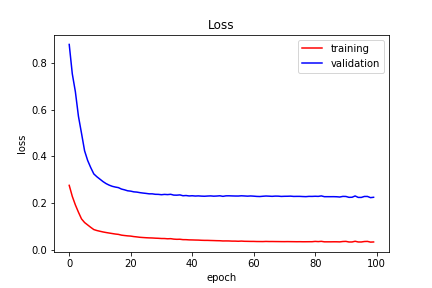
\includegraphics[width=\linewidth]{images/trained_online_lstm/tile_by_tile_training_uniform_random_fill_10000_model_loss.png}
     \caption{Training/Validation Loss}
  \end{subfigure}
  \hfill
  \begin{subfigure}[b]{0.35\linewidth}
    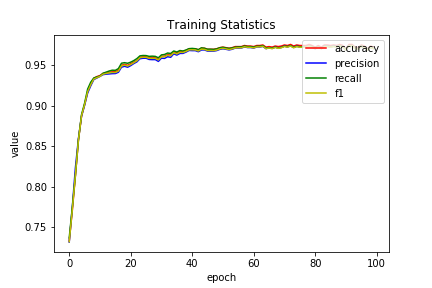
\includegraphics[width=\linewidth]{images/trained_online_lstm/tile_by_tile_training_uniform_random_fill_10000_model_training_stats.png}
     \caption{Training Statistics}
  \end{subfigure}
  \hfill
  \begin{subfigure}[b]{0.35\linewidth}
    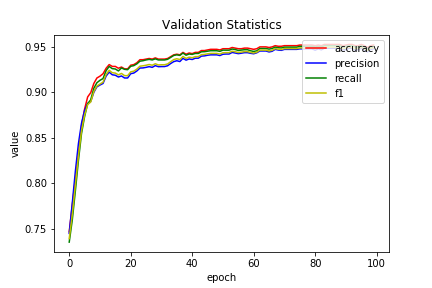
\includegraphics[width=\linewidth]{images/trained_online_lstm/tile_by_tile_training_uniform_random_fill_10000_model_validation_stats.png}
     \caption{Validation Statistics}
  \end{subfigure}
  \caption{Training statistics for Algorithm \hyperref[tab: app_evalalgorithms]{1}}
  \label{fig: train_olnine_lstm_1}
\end{figure}

\begin{figure}[h!]
  \centerfloat
  \begin{subfigure}[b]{0.35\linewidth}
    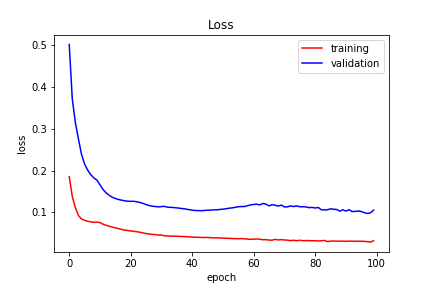
\includegraphics[width=\linewidth]{images/trained_online_lstm/tile_by_tile_training_block_map_10000_model_loss.png}
     \caption{Training/Validation Loss}
  \end{subfigure}
  \hfill
  \begin{subfigure}[b]{0.35\linewidth}
    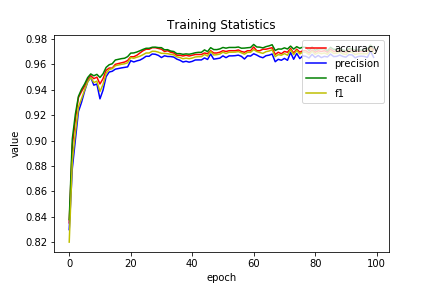
\includegraphics[width=\linewidth]{images/trained_online_lstm/tile_by_tile_training_block_map_10000_model_training_stats.png}
     \caption{Training Statistics}
  \end{subfigure}
  \hfill
  \begin{subfigure}[b]{0.35\linewidth}
    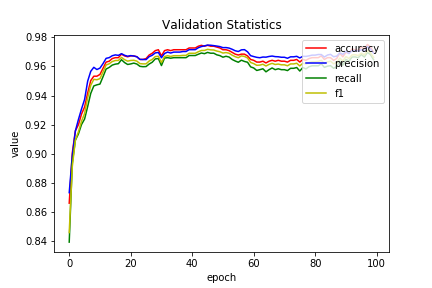
\includegraphics[width=\linewidth]{images/trained_online_lstm/tile_by_tile_training_block_map_10000_model_validation_stats.png}
     \caption{Validation Statistics}
  \end{subfigure}
  \caption{Training statistics for Algorithm \hyperref[tab: app_evalalgorithms]{2}}
  \label{fig: train_olnine_lstm_2}
\end{figure}

\begin{figure}[h!]
  \centerfloat
  \begin{subfigure}[b]{0.35\linewidth}
    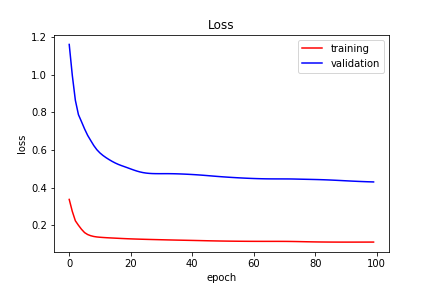
\includegraphics[width=\linewidth]{images/trained_online_lstm/tile_by_tile_training_house_10000_model_loss.png}
     \caption{Training/Validation Loss}
  \end{subfigure}
  \hfill
  \begin{subfigure}[b]{0.35\linewidth}
    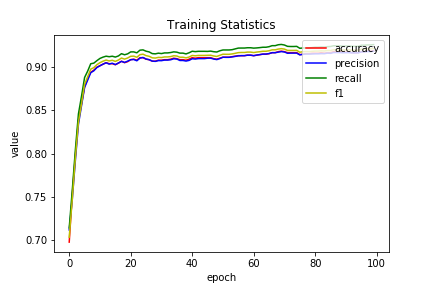
\includegraphics[width=\linewidth]{images/trained_online_lstm/tile_by_tile_training_house_10000_model_training_stats.png}
     \caption{Training Statistics}
  \end{subfigure}
  \hfill
  \begin{subfigure}[b]{0.35\linewidth}
    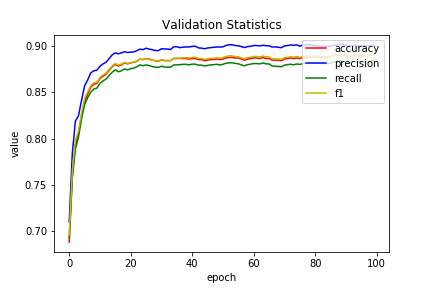
\includegraphics[width=\linewidth]{images/trained_online_lstm/tile_by_tile_training_house_10000_model_validation_stats.png}
     \caption{Validation Statistics}
  \end{subfigure}
  \caption{Training statistics for Algorithm \hyperref[tab: app_evalalgorithms]{3}}
  \label{fig: train_olnine_lstm_3}
\end{figure}

\begin{figure}[h!]
  \centerfloat
  \begin{subfigure}[b]{0.35\linewidth}
    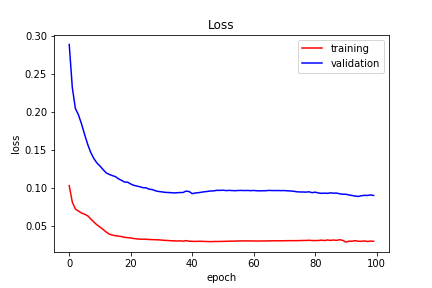
\includegraphics[width=\linewidth]{images/trained_online_lstm/tile_by_tile_training_uniform_random_fill_10000_block_map_10000_model_loss.png}
     \caption{Training/Validation Loss}
  \end{subfigure}
  \hfill
  \begin{subfigure}[b]{0.35\linewidth}
    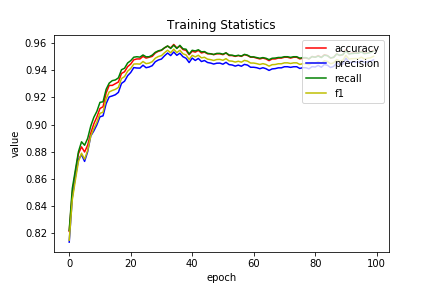
\includegraphics[width=\linewidth]{images/trained_online_lstm/tile_by_tile_training_uniform_random_fill_10000_block_map_10000_model_training_stats.png}
     \caption{Training Statistics}
  \end{subfigure}
  \hfill
  \begin{subfigure}[b]{0.35\linewidth}
    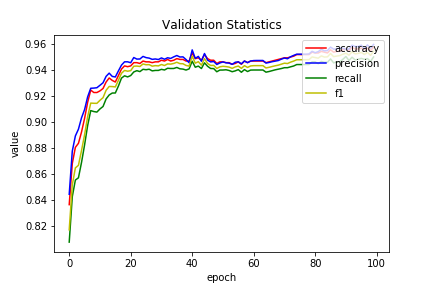
\includegraphics[width=\linewidth]{images/trained_online_lstm/tile_by_tile_training_uniform_random_fill_10000_block_map_10000_model_validation_stats.png}
     \caption{Validation Statistics}
  \end{subfigure}
  \caption{Training statistics for Algorithm \hyperref[tab: app_evalalgorithms]{4}}
  \label{fig: train_olnine_lstm_4}
\end{figure}

\pagebreak

\begin{figure}[h!]
  \centerfloat
  \begin{subfigure}[b]{0.35\linewidth}
    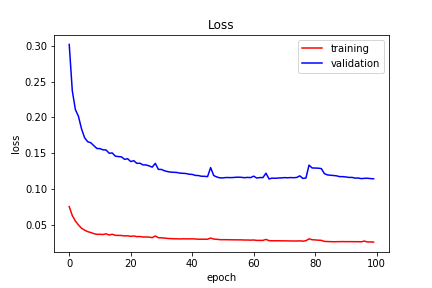
\includegraphics[width=\linewidth]{images/trained_online_lstm/tile_by_tile_training_uniform_random_fill_10000_block_map_10000_house_10000_model_loss.png}
     \caption{Training/Validation Loss}
  \end{subfigure}
  \hfill
  \begin{subfigure}[b]{0.35\linewidth}
    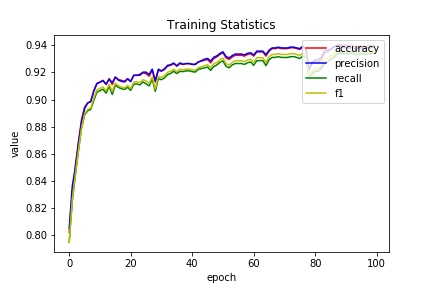
\includegraphics[width=\linewidth]{images/trained_online_lstm/tile_by_tile_training_uniform_random_fill_10000_block_map_10000_house_10000_model_training_stats.png}
     \caption{Training Statistics}
  \end{subfigure}
  \hfill
  \begin{subfigure}[b]{0.35\linewidth}
    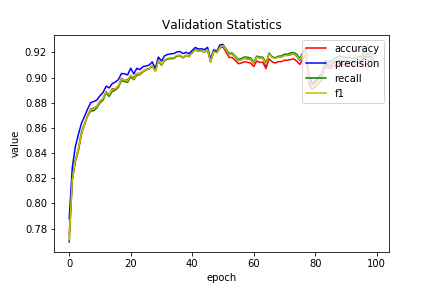
\includegraphics[width=\linewidth]{images/trained_online_lstm/tile_by_tile_training_uniform_random_fill_10000_block_map_10000_house_10000_model_validation_stats.png}
     \caption{Validation Statistics}
  \end{subfigure}
  \caption{Training statistics for Algorithm \hyperref[tab: app_evalalgorithms]{5}}
  \label{fig: train_olnine_lstm_5}
\end{figure}

\clearpage

\section{CAE Online LSTM Planner Full Training Analysis}
% algo 6

\begin{figure}[h!]
    \centerfloat
    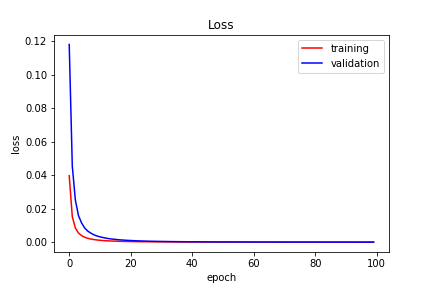
\includegraphics[scale=0.6]{images/cae_online_lstm/caelstm_section_cae_training_uniform_random_fill_10000_model_loss.png}
    \caption{Training/Validation Loss for CAE model (Algorithm \hyperref[tab: app_evalalgorithms]{6}) training loss (Train Loss: 0.000002, Validation Loss: 0.000005, Evaluation Loss: 0.000005)}
    \label{fig: cae_6_train}
\end{figure}

\begin{figure}[h!]
    \centerfloat
    \begin{subfigure}[b]{1.25\linewidth}
        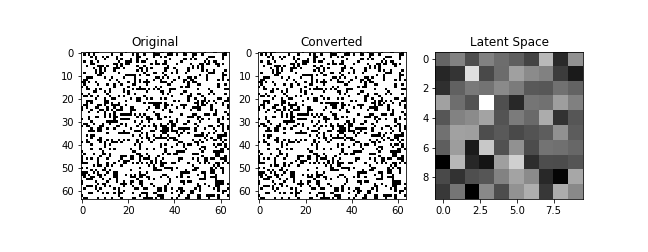
\includegraphics[width=\linewidth]{images/cae_online_lstm/caelstm_section_cae_training_uniform_random_fill_10000_model_network_analysis_0.png}
    \end{subfigure}
    \\[-1.5cm]
    \begin{subfigure}[b]{1.25\linewidth}
        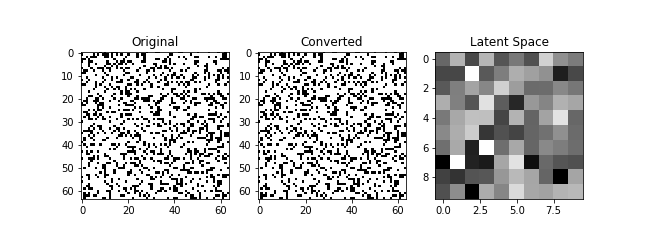
\includegraphics[width=\linewidth]{images/cae_online_lstm/caelstm_section_cae_training_uniform_random_fill_10000_model_network_analysis_1.png}
    \end{subfigure}
    
    \caption{CAE model (Algorithm \hyperref[tab: app_evalalgorithms]{6}) network analysis}
    \label{fig: cae_6_net_analysis}
\end{figure}

\pagebreak

\begin{figure}
    \centering
    \begin{subfigure}[b]{0.40\linewidth}
        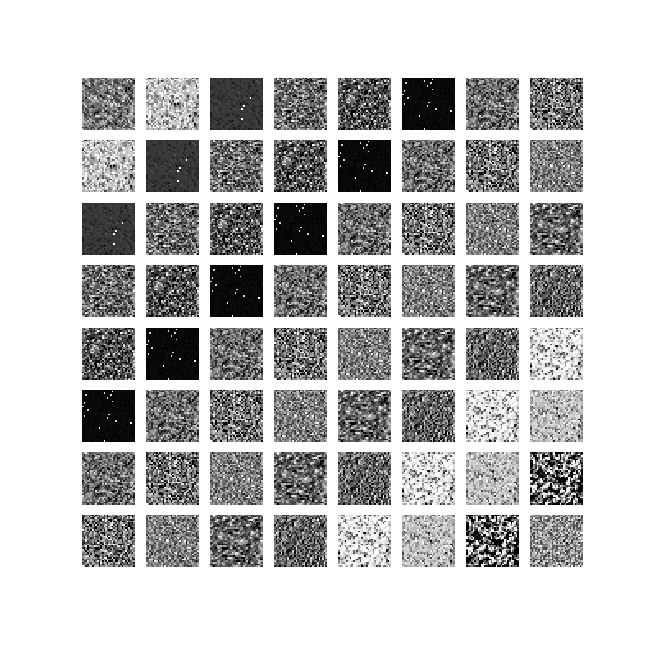
\includegraphics[width=\linewidth]{images/cae_online_lstm/caelstm_section_cae_training_uniform_random_fill_10000_model_feature_maps_map_0_0_3.png}
    \end{subfigure}
    \hfill
    \begin{subfigure}[b]{0.40\linewidth}
        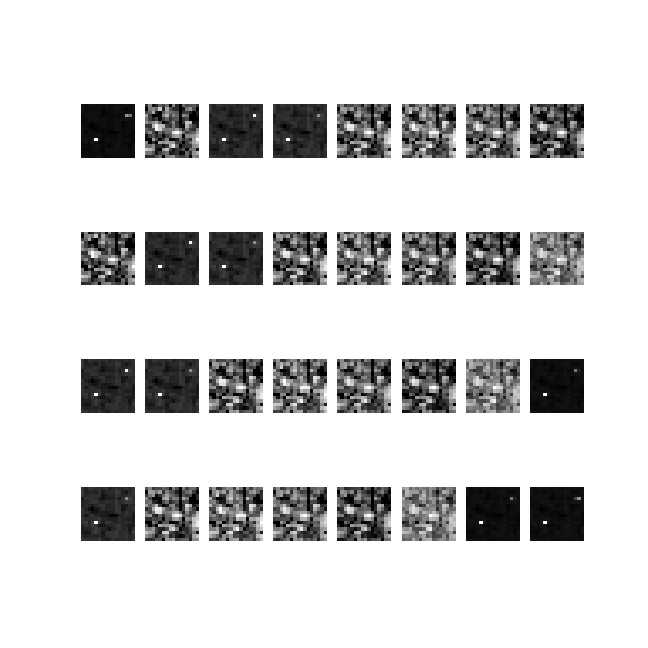
\includegraphics[width=\linewidth]{images/cae_online_lstm/caelstm_section_cae_training_uniform_random_fill_10000_model_feature_maps_map_0_0_2.png}
    \end{subfigure}
    \\[-0.5cm]
    \begin{subfigure}[b]{0.40\linewidth}
        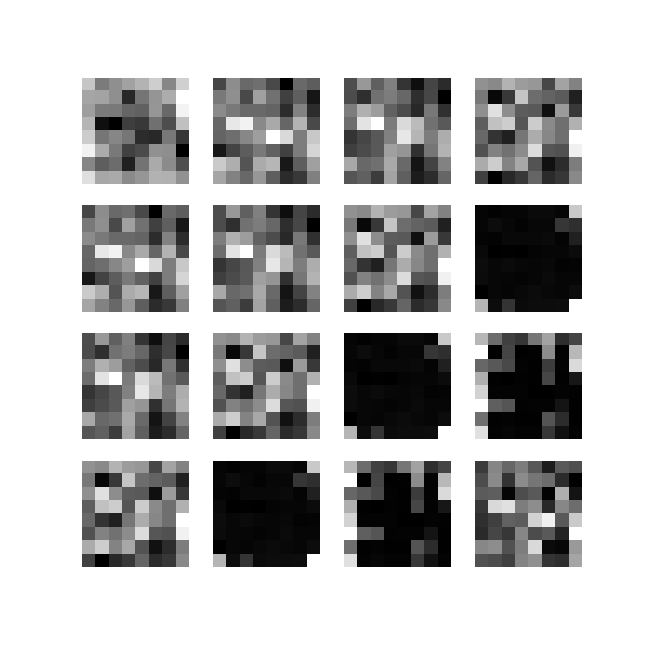
\includegraphics[width=\linewidth]{images/cae_online_lstm/caelstm_section_cae_training_uniform_random_fill_10000_model_feature_maps_map_0_0_1.png}
    \end{subfigure}
    \hfill
    \begin{subfigure}[b]{0.40\linewidth}
        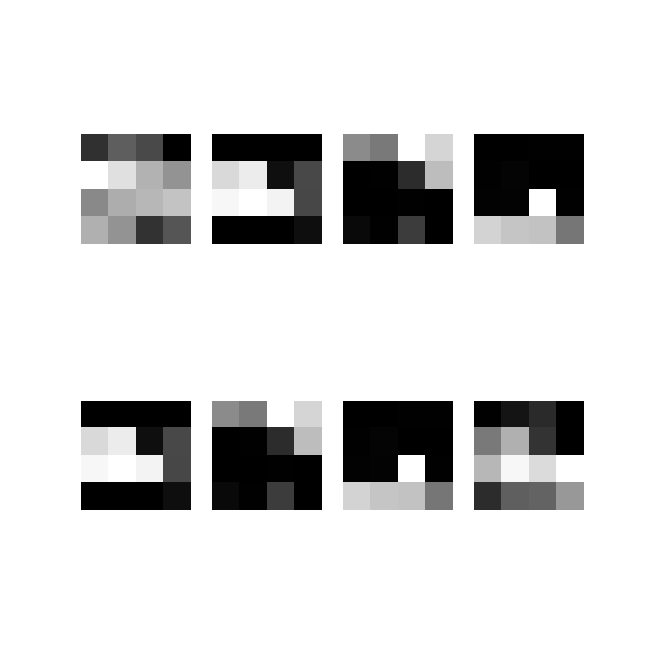
\includegraphics[width=\linewidth]{images/cae_online_lstm/caelstm_section_cae_training_uniform_random_fill_10000_model_feature_maps_map_0_0_0.png}
    \end{subfigure}
    \\[-0.5cm]
    \caption{CAE model (Algorithm \hyperref[tab: app_evalalgorithms]{6}) first map from Figure \ref{fig: cae_6_net_analysis} feature maps}
    \label{fig: cae_6_feature_maps_1}
\end{figure}

\begin{figure}
    \centering
    \begin{subfigure}[b]{0.4\linewidth}
        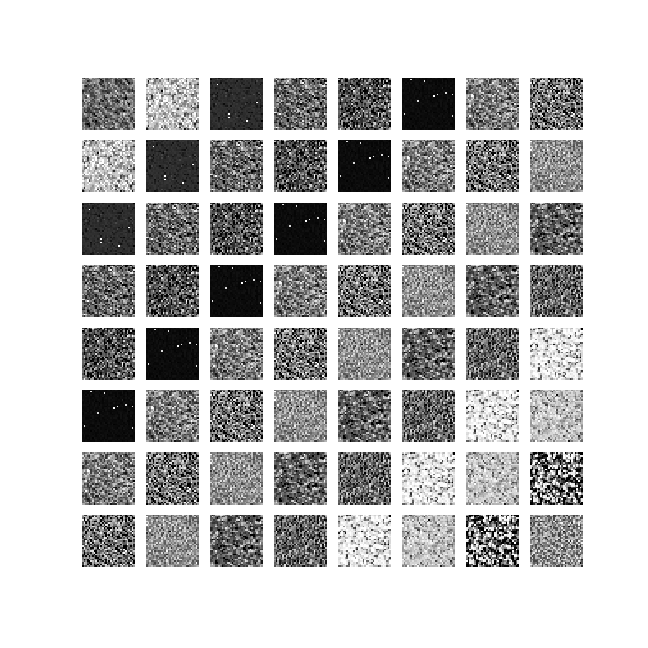
\includegraphics[width=\linewidth]{images/cae_online_lstm/caelstm_section_cae_training_uniform_random_fill_10000_model_feature_maps_map_1_0_3.png}
    \end{subfigure}
    \hfill
    \begin{subfigure}[b]{0.4\linewidth}
        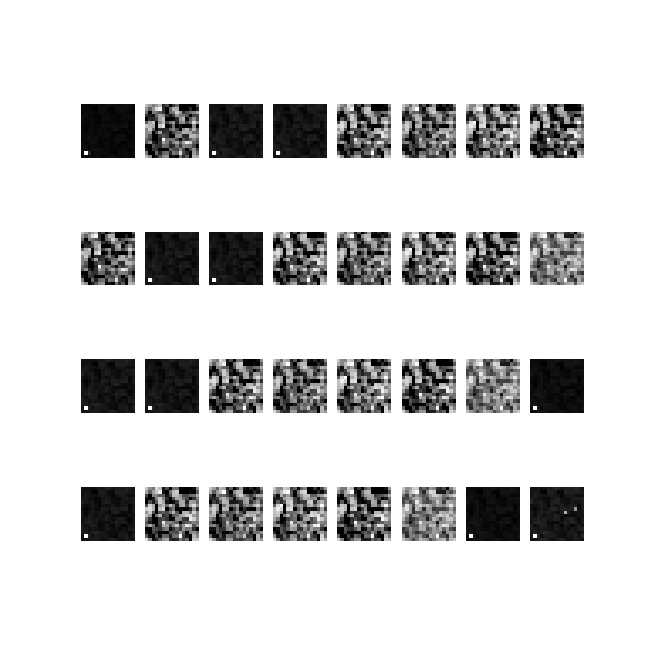
\includegraphics[width=\linewidth]{images/cae_online_lstm/caelstm_section_cae_training_uniform_random_fill_10000_model_feature_maps_map_1_0_2.png}
    \end{subfigure}
    \\[-0.5cm]
    \begin{subfigure}[b]{0.4\linewidth}
        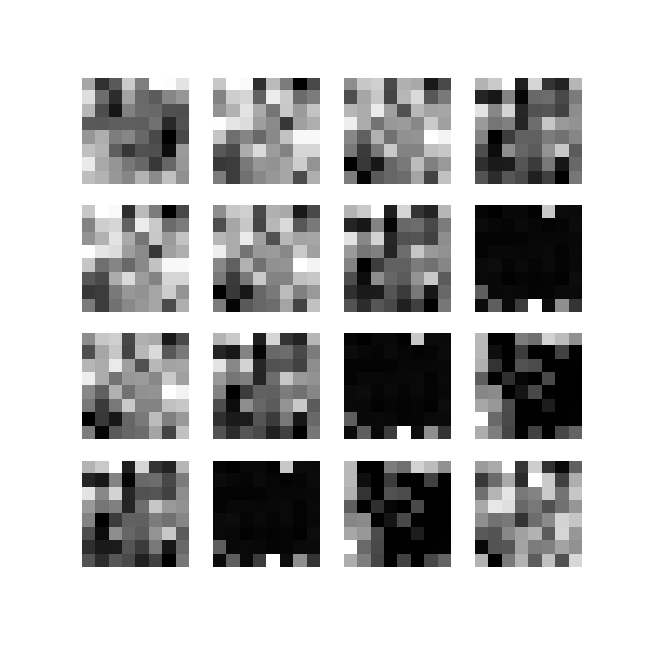
\includegraphics[width=\linewidth]{images/cae_online_lstm/caelstm_section_cae_training_uniform_random_fill_10000_model_feature_maps_map_1_0_1.png}
    \end{subfigure}
    \hfill
    \begin{subfigure}[b]{0.4\linewidth}
        
\includegraphics[width=\linewidth]{images/cae_online_lstm/caelstm_section_cae_training_uniform_random_fill_10000_model_feature_maps_map_1_0_0.png}
    \end{subfigure}
    \\[-0.5cm]
    \caption{CAE model (Algorithm \hyperref[tab: app_evalalgorithms]{6}) second map from Figure \ref{fig: cae_6_net_analysis} feature maps}
    \label{fig: cae_6_feature_maps_2}
\end{figure}

% algo 7

\begin{figure}
    \centerfloat
    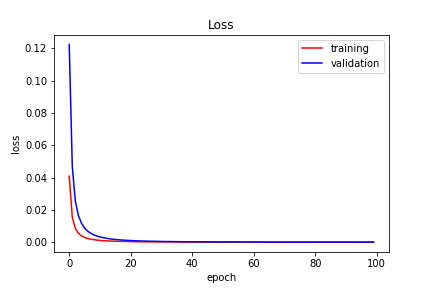
\includegraphics[scale=0.6]{images/cae_online_lstm/caelstm_section_cae_training_block_map_10000_model_loss.png}
    \caption{Training/Validation Loss for CAE model (Algorithm \hyperref[tab: app_evalalgorithms]{7}) (Train Loss: 0.000002, Validation Loss: 0.000005, Evaluation Loss: 0.000005)}
    \label{fig: cae_7_train}
\end{figure}

\begin{figure}
    \centerfloat
    \begin{subfigure}[b]{1.25\linewidth}
        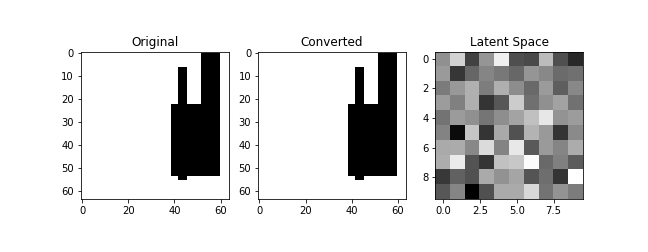
\includegraphics[width=\linewidth]{images/cae_online_lstm/caelstm_section_cae_training_block_map_10000_model_network_analysis_0.png}
    \end{subfigure}
    \\[-1.5cm]
    \begin{subfigure}[b]{1.25\linewidth}
        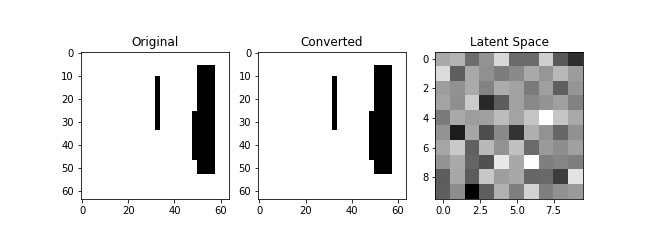
\includegraphics[width=\linewidth]{images/cae_online_lstm/caelstm_section_cae_training_block_map_10000_model_network_analysis_1.png}
    \end{subfigure}
    
    \caption{CAE model (Algorithm \hyperref[tab: app_evalalgorithms]{7}) network analysis}
    \label{fig: cae_7_net_analysis}
\end{figure}

\begin{figure}
    \centering
    \begin{subfigure}[b]{0.40\linewidth}
        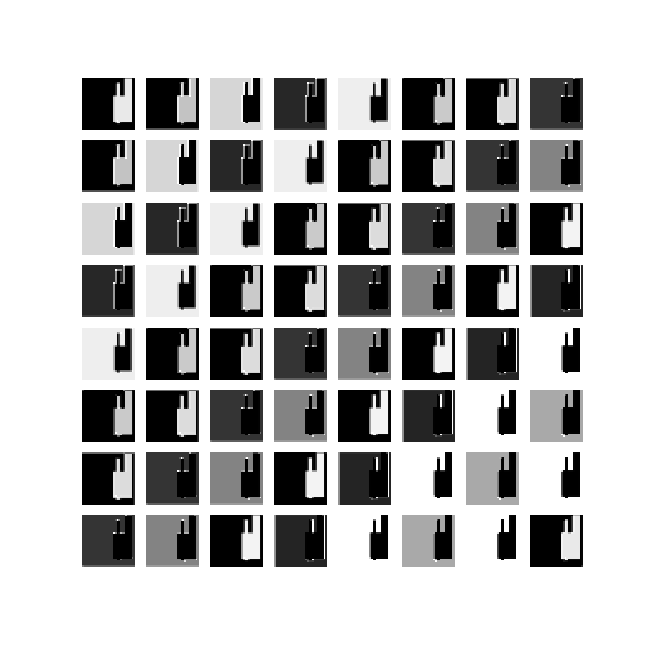
\includegraphics[width=\linewidth]{images/cae_online_lstm/caelstm_section_cae_training_block_map_10000_model_feature_maps_map_0_0_3.png}
    \end{subfigure}
    \hfill
    \begin{subfigure}[b]{0.40\linewidth}
        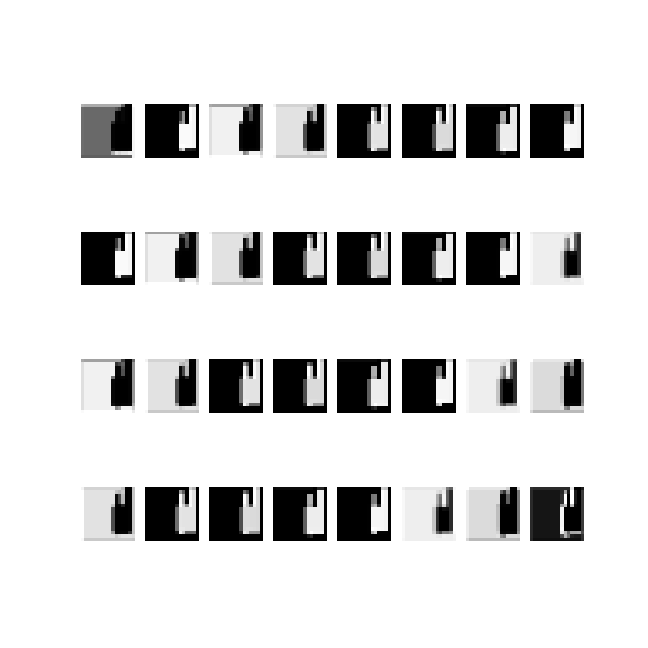
\includegraphics[width=\linewidth]{images/cae_online_lstm/caelstm_section_cae_training_block_map_10000_model_feature_maps_map_0_0_2.png}
    \end{subfigure}
    \\[-0.5cm]
    \begin{subfigure}[b]{0.40\linewidth}
        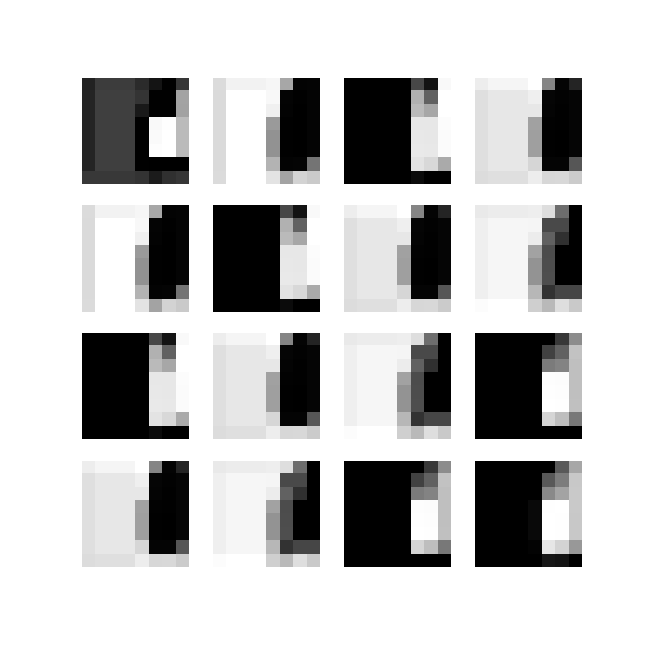
\includegraphics[width=\linewidth]{images/cae_online_lstm/caelstm_section_cae_training_block_map_10000_model_feature_maps_map_0_0_1.png}
    \end{subfigure}
    \hfill
    \begin{subfigure}[b]{0.40\linewidth}
        
\includegraphics[width=\linewidth]{images/cae_online_lstm/caelstm_section_cae_training_block_map_10000_model_feature_maps_map_0_0_0.png}
    \end{subfigure}
    \\[-0.5cm]
    \caption{CAE model (Algorithm \hyperref[tab: app_evalalgorithms]{7}) first map from Figure \ref{fig: cae_7_net_analysis} feature maps}
    \label{fig: cae_7_feature_maps_1}
\end{figure}

\begin{figure}
    \centering
    \begin{subfigure}[b]{0.4\linewidth}
        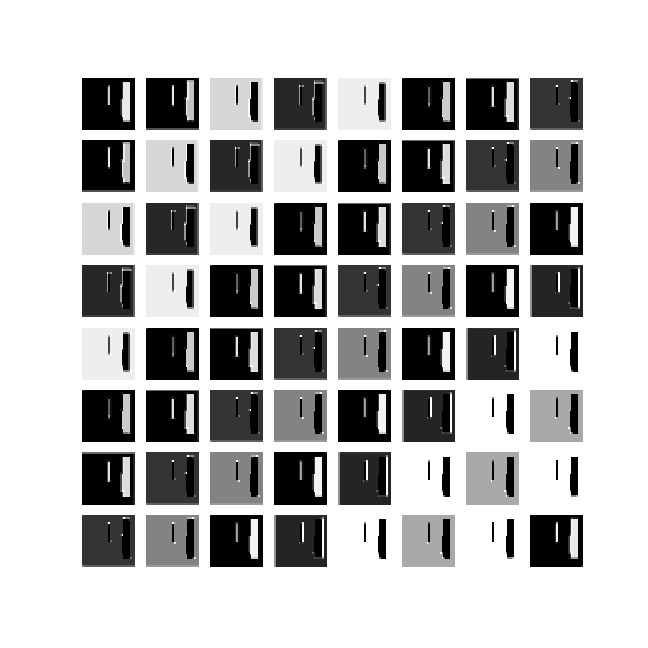
\includegraphics[width=\linewidth]{images/cae_online_lstm/caelstm_section_cae_training_block_map_10000_model_feature_maps_map_1_0_3.png}
    \end{subfigure}
    \hfill
    \begin{subfigure}[b]{0.4\linewidth}
        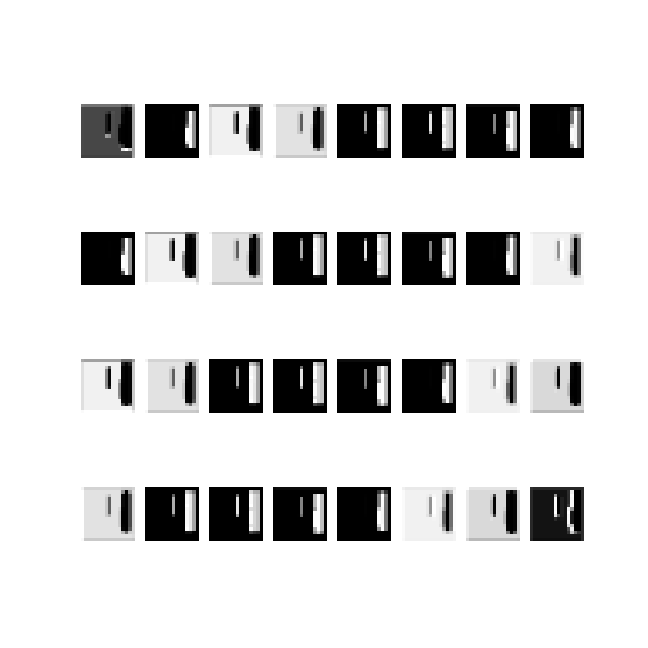
\includegraphics[width=\linewidth]{images/cae_online_lstm/caelstm_section_cae_training_block_map_10000_model_feature_maps_map_1_0_2.png}
    \end{subfigure}
    \\[-0.5cm]
    \begin{subfigure}[b]{0.4\linewidth}
        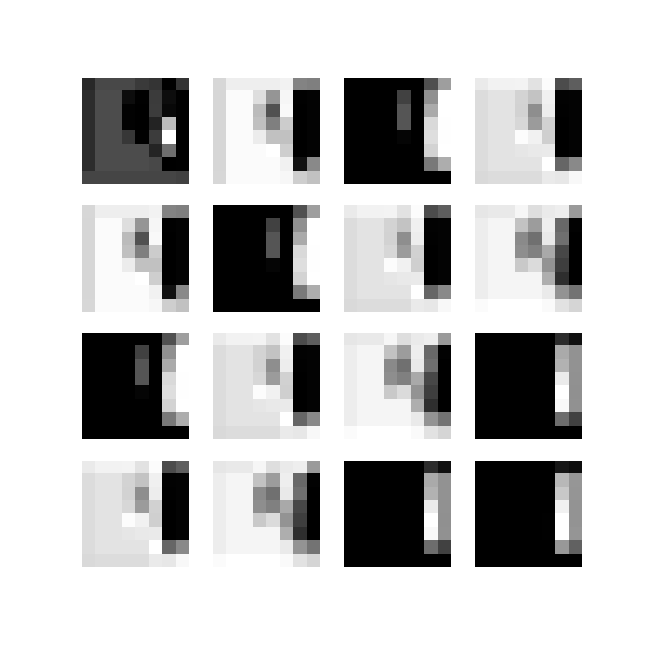
\includegraphics[width=\linewidth]{images/cae_online_lstm/caelstm_section_cae_training_block_map_10000_model_feature_maps_map_1_0_1.png}
    \end{subfigure}
    \hfill
    \begin{subfigure}[b]{0.4\linewidth}
        
\includegraphics[width=\linewidth]{images/cae_online_lstm/caelstm_section_cae_training_block_map_10000_model_feature_maps_map_1_0_0.png}
    \end{subfigure}
    \\[-0.5cm]
    \caption{CAE model (Algorithm \hyperref[tab: app_evalalgorithms]{7}) second map from Figure \ref{fig: cae_7_net_analysis} feature maps}
    \label{fig: cae_7_feature_maps_2}
\end{figure}

% algo 8

\begin{figure}
    \centerfloat
    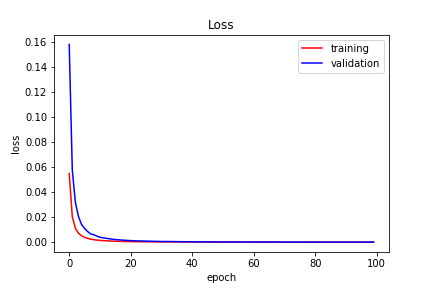
\includegraphics[scale=0.6]{images/cae_online_lstm/caelstm_section_cae_training_house_10000_model_loss.png}
    \caption{Training/Validation Loss for CAE model (Algorithm \hyperref[tab: app_evalalgorithms]{8}) (Train Loss: 0.000002, Validation Loss: 0.000007, Evaluation Loss: 0.000007)}
    \label{fig: cae_8_train}
\end{figure}

\begin{figure}
    \centerfloat
    \begin{subfigure}[b]{1.25\linewidth}
        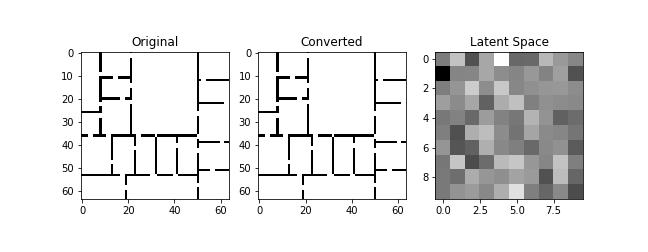
\includegraphics[width=\linewidth]{images/cae_online_lstm/caelstm_section_cae_training_house_10000_model_network_analysis_0.png}
    \end{subfigure}
    \\[-1.5cm]
    \begin{subfigure}[b]{1.25\linewidth}
        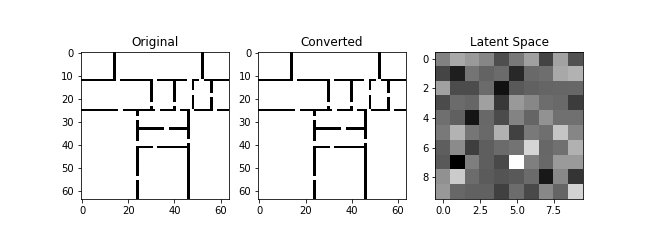
\includegraphics[width=\linewidth]{images/cae_online_lstm/caelstm_section_cae_training_house_10000_model_network_analysis_1.png}
    \end{subfigure}
    
    \caption{CAE model (Algorithm \hyperref[tab: app_evalalgorithms]{8}) network analysis}
    \label{fig: cae_8_net_analysis}
\end{figure}

\begin{figure}
    \centering
    \begin{subfigure}[b]{0.40\linewidth}
        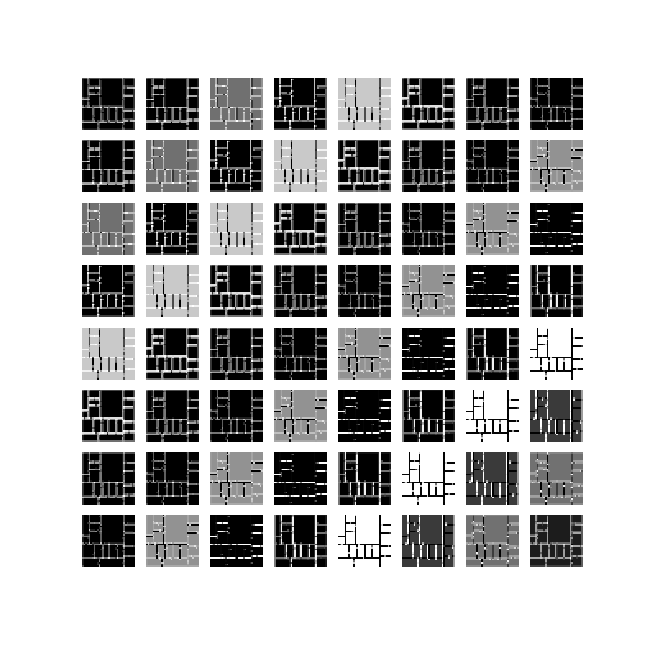
\includegraphics[width=\linewidth]{images/cae_online_lstm/caelstm_section_cae_training_house_10000_model_feature_maps_map_0_0_3.png}
    \end{subfigure}
    \hfill
    \begin{subfigure}[b]{0.40\linewidth}
        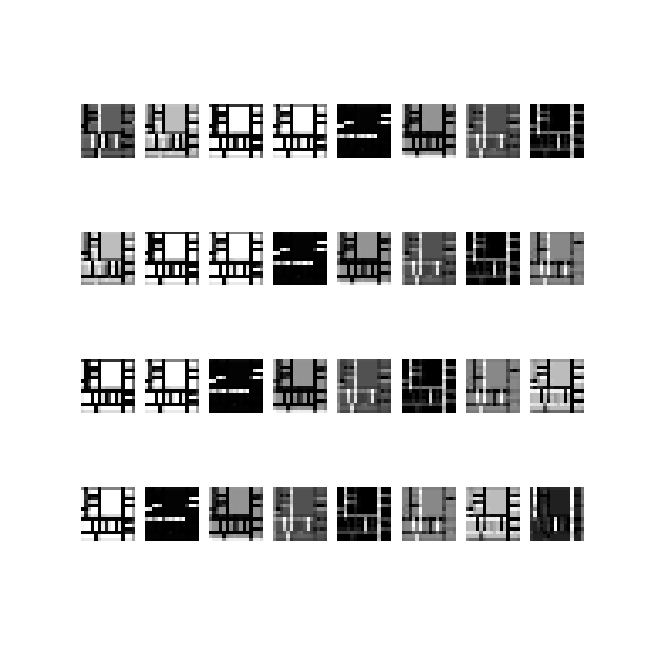
\includegraphics[width=\linewidth]{images/cae_online_lstm/caelstm_section_cae_training_house_10000_model_feature_maps_map_0_0_2.png}
    \end{subfigure}
    \\[-0.5cm]
    \begin{subfigure}[b]{0.40\linewidth}
        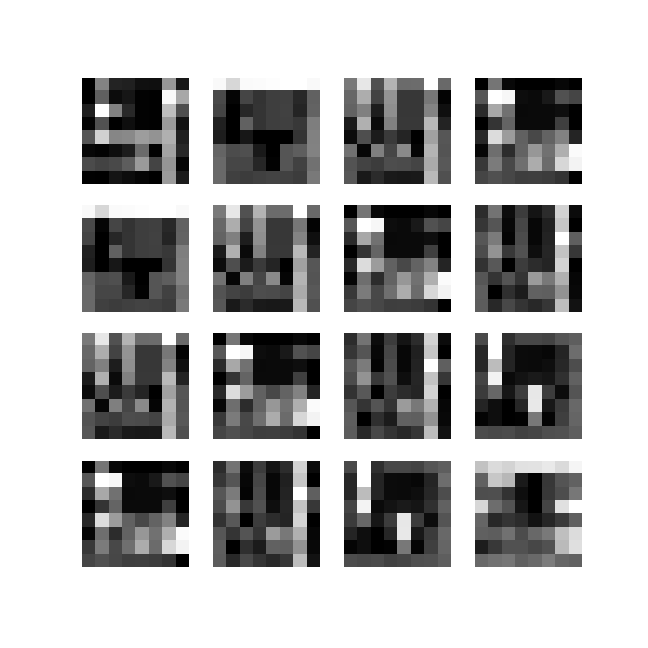
\includegraphics[width=\linewidth]{images/cae_online_lstm/caelstm_section_cae_training_house_10000_model_feature_maps_map_0_0_1.png}
    \end{subfigure}
    \hfill
    \begin{subfigure}[b]{0.40\linewidth}
        
\includegraphics[width=\linewidth]{images/cae_online_lstm/caelstm_section_cae_training_house_10000_model_feature_maps_map_0_0_0.png}
    \end{subfigure}
    \\[-0.5cm]
    \caption{CAE model (Algorithm \hyperref[tab: app_evalalgorithms]{8}) first map from Figure \ref{fig: cae_8_net_analysis} feature maps}
    \label{fig: cae_8_feature_maps_1}
\end{figure}

\begin{figure}
    \centering
    \begin{subfigure}[b]{0.4\linewidth}
        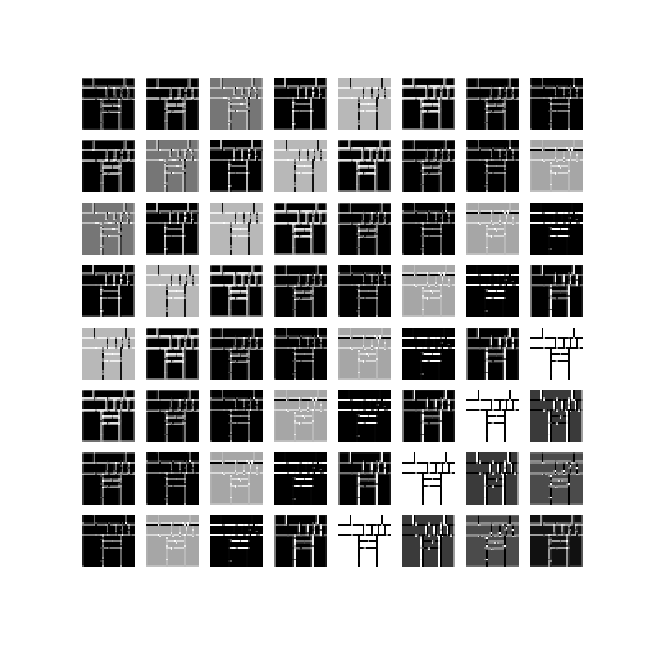
\includegraphics[width=\linewidth]{images/cae_online_lstm/caelstm_section_cae_training_house_10000_model_feature_maps_map_1_0_3.png}
    \end{subfigure}
    \hfill
    \begin{subfigure}[b]{0.4\linewidth}
        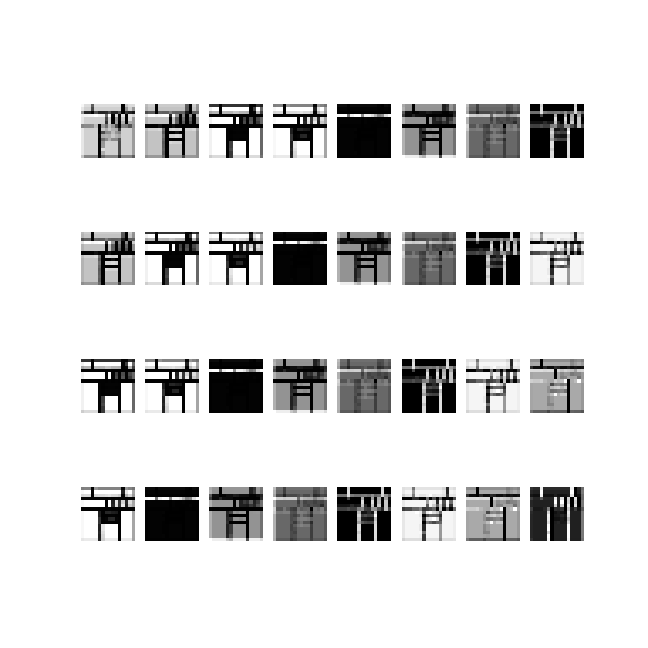
\includegraphics[width=\linewidth]{images/cae_online_lstm/caelstm_section_cae_training_house_10000_model_feature_maps_map_1_0_2.png}
    \end{subfigure}
    \\[-0.5cm]
    \begin{subfigure}[b]{0.4\linewidth}
        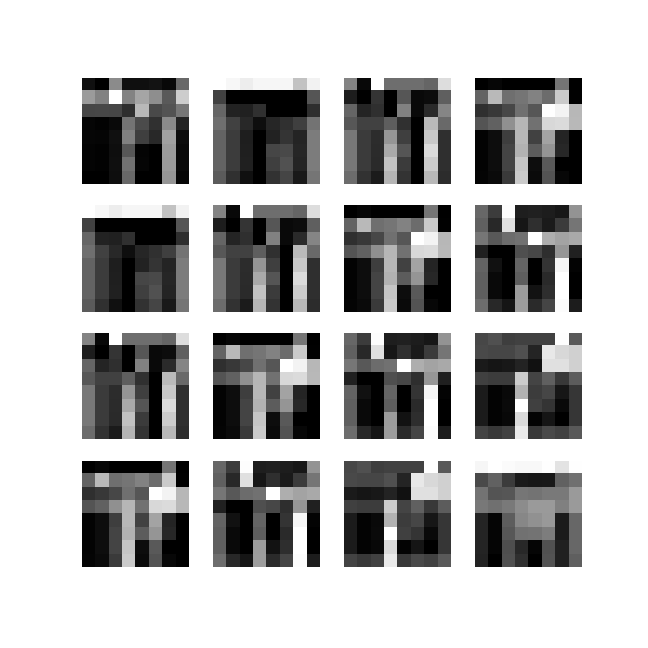
\includegraphics[width=\linewidth]{images/cae_online_lstm/caelstm_section_cae_training_house_10000_model_feature_maps_map_1_0_1.png}
    \end{subfigure}
    \hfill
    \begin{subfigure}[b]{0.4\linewidth}
        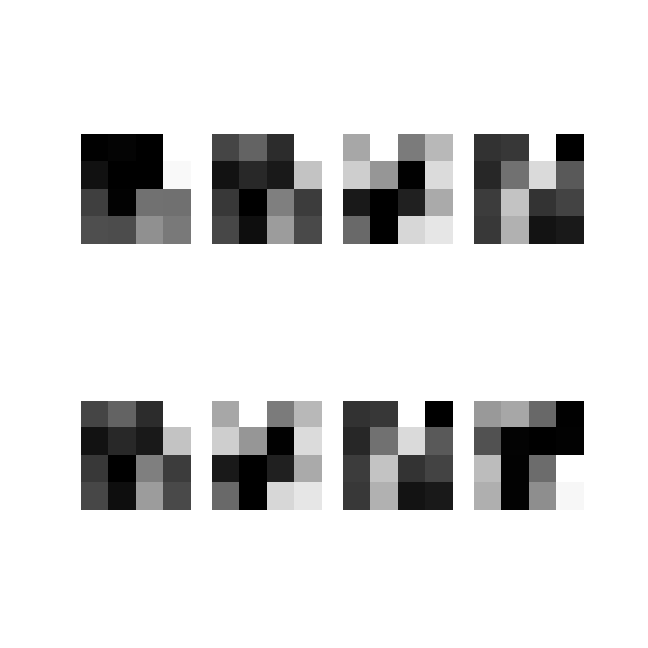
\includegraphics[width=\linewidth]{images/cae_online_lstm/caelstm_section_cae_training_house_10000_model_feature_maps_map_1_0_0.png}
    \end{subfigure}
    \\[-0.5cm]
    \caption{CAE model (Algorithm \hyperref[tab: app_evalalgorithms]{8}) second map from Figure \ref{fig: cae_8_net_analysis} feature maps}
    \label{fig: cae_8_feature_maps_2}
\end{figure}

\clearpage

\begin{table}[h!]
    \footnotesize
    \centerfloat
    \begin{tabular}{|c|c|M{1.3cm}|M{1.5cm}|M{1.5cm}|c|c|c|c|M{0.7cm}|}
         \hline
         \textbf{Model} & \textbf{Epochs} & \textbf{Training Loss} & \textbf{Validation Loss} & \textbf{Evaluation Loss} & \textbf{Accuracy} & \textbf{Precision} & \textbf{Recall} & \textbf{F1} & \textbf{CM} \\
         \hline
         \cellcolor{blue!20}\hyperref[tab: evalalgorithms]{6} & 34 & 0.042641 & 0.153901 & 0.178480 & 0.96 & 0.96 & 0.95 & 0.95 & See Table \ref{tab: cm_online_lstm_6} \\
         \hline
         \cellcolor{blue!40}\hyperref[tab: evalalgorithms]{7} & 25 & 0.031109 & 0.169480 & 0.145604 & 0.96 & 0.96  & 0.95 & 0.95 & See Table \ref{tab: cm_online_lstm_7} \\
         \hline
         \cellcolor{blue!20}\hyperref[tab: evalalgorithms]{8} & 45 & 0.146206 & 0.393990 & 0.610441 & 0.87 & 0.88 & 0.88 & 0.88 & See Table \ref{tab: cm_online_lstm_8} \\
         \hline
         \cellcolor{blue!20}\hyperref[tab: evalalgorithms]{9} & 37 & 0.019767 & 0.066242 & 0.097563 & 0.95 & 0.95 & 0.94 & 0.94 & See Table \ref{tab: cm_online_lstm_9} \\
         \hline
         \cellcolor{blue!20}\hyperref[tab: evalalgorithms]{10} & 50 & 0.033152 & 0.118695 & 0.096448 & 0.92 & 0.92 & 0.92 & 0.92 & See Table \ref{tab: cm_online_lstm_10} \\
         \hline
    \end{tabular}
    \caption{CAE Online LSTM Planner final training statistics (CM is short-hand for Confusion Matrix)}
    \label{tab: cae_online_lstm_final_tr_res}
\end{table}

\begin{table}[h!]
\centering
\small
    \begin{tabular}{|c|c|cccccccc|} 
    \hline & \multicolumn{9}{c|}{\textbf{Predicted}} \\ 
    \hline
    \multirow{9}{*}{\rotatebox{90}{\textbf{Actual}}} & \textbf{Action} & \multicolumn{1}{c|}{0} & \multicolumn{1}{c|}{1} & \multicolumn{1}{c|}{2} & \multicolumn{1}{c|}{3} & \multicolumn{1}{c|}{4} & \multicolumn{1}{c|}{5} & \multicolumn{1}{c|}{6} & 7  \\ 
    \cline{2-10} & \multicolumn{1}{c|}{0} & 217 &   2 &   0 &   1 &   0 &   0 &   0 &   2  \\
    \cline{2-2}  & \multicolumn{1}{c|}{1} &   2 & 243 &   5 &   3 &   0 &   0 &   0 &   2  \\
    \cline{2-2}  & \multicolumn{1}{c|}{2} &   0 &   2 & 109 &   3 &   1 &   0 &   0 &   0  \\
    \cline{2-2}  & \multicolumn{1}{c|}{3} &   0 &   0 &   2 & 143 &   1 &   0 &   0 &   0  \\
    \cline{2-2}  & \multicolumn{1}{c|}{4} &   0 &   0 &   1 &   1 & 174 &   1 &   3 &   1  \\
    \cline{2-2}  & \multicolumn{1}{c|}{5} &   0 &   0 &   0 &   1 &   0 & 235 &   2 &   3  \\
    \cline{2-2}  & \multicolumn{1}{c|}{6} &   7 &   1 &   0 &   0 &   1 &   1 & 121 &   5  \\
    \cline{2-2}  & \multicolumn{1}{c|}{7} &   2 &   3 &   0 &   0 &   0 &   0 &   0 & 313  \\
    \hline
    \end{tabular}
    \caption{Confusion matrix for Algorithm \hyperref[tab: app_evalalgorithms]{6}}
        \label{tab: cm_online_lstm_6}
\end{table}

\begin{table}[h!]
\centering
\small
    \begin{tabular}{|c|c|cccccccc|} 
    \hline & \multicolumn{9}{c|}{\textbf{Predicted}} \\ 
    \hline
    \multirow{9}{*}{\rotatebox{90}{\textbf{Actual}}} & \textbf{Action} & \multicolumn{1}{c|}{0} & \multicolumn{1}{c|}{1} & \multicolumn{1}{c|}{2} & \multicolumn{1}{c|}{3} & \multicolumn{1}{c|}{4} & \multicolumn{1}{c|}{5} & \multicolumn{1}{c|}{6} & 7  \\ 
    \cline{2-10} & \multicolumn{1}{c|}{0} & 294 &   1 &   0 &   0 &   4 &   0 &   0 &   0 \\
    \cline{2-2}  & \multicolumn{1}{c|}{1} &   2 & 106 &   3 &   1 &   0 &   0 &   0 &   2 \\
    \cline{2-2}  & \multicolumn{1}{c|}{2} &   0 &   0 & 235 &   0 &   0 &   0 &  11 &   0 \\
    \cline{2-2}  & \multicolumn{1}{c|}{3} &   0 &   0 &   0 & 130 &   2 &   0 &   0 &   0 \\
    \cline{2-2}  & \multicolumn{1}{c|}{4} &   5 &   0 &   0 &   1 & 186 &   0 &   0 &   0 \\
    \cline{2-2}  & \multicolumn{1}{c|}{5} &   0 &   0 &   0 &   5 &   4 & 192 &   3 &   1 \\
    \cline{2-2}  & \multicolumn{1}{c|}{6} &   0 &   0 &   3 &   0 &   0 &   1 & 396 &   2 \\
    \cline{2-2}  & \multicolumn{1}{c|}{7} &   3 &   5 &   1 &   0 &   0 &   0 &  10 & 194 \\
    \hline
    \end{tabular}
    \caption{Confusion matrix for Algorithm \hyperref[tab: app_evalalgorithms]{7}}
        \label{tab: cm_online_lstm_7}
\end{table}

\begin{table}[h!]
\centering
\small
    \begin{tabular}{|c|c|cccccccc|} 
    \hline & \multicolumn{9}{c|}{\textbf{Predicted}} \\ 
    \hline
    \multirow{9}{*}{\rotatebox{90}{\textbf{Actual}}} & \textbf{Action} & \multicolumn{1}{c|}{0} & \multicolumn{1}{c|}{1} & \multicolumn{1}{c|}{2} & \multicolumn{1}{c|}{3} & \multicolumn{1}{c|}{4} & \multicolumn{1}{c|}{5} & \multicolumn{1}{c|}{6} & 7  \\ 
    \cline{2-10} & \multicolumn{1}{c|}{0} & 148 &   2 &   0 &   0 &   0 &   1 &   0 &   4  \\
    \cline{2-2}  & \multicolumn{1}{c|}{1} &   1 & 255 &   3 &   4 &   0 &  10 &   2 &   6  \\
    \cline{2-2}  & \multicolumn{1}{c|}{2} &   0 &  15 & 116 &   6 &   0 &   1 &  10 &   4  \\
    \cline{2-2}  & \multicolumn{1}{c|}{3} &   0 &  16 &   4 & 222 &   6 &   9 &   4 &   5  \\
    \cline{2-2}  & \multicolumn{1}{c|}{4} &  10 &   1 &   0 &   2 & 217 &   8 &   0 &   0  \\
    \cline{2-2}  & \multicolumn{1}{c|}{5} &   0 &   2 &   0 &  10 &   6 & 250 &   5 &  20  \\
    \cline{2-2}  & \multicolumn{1}{c|}{6} &   0 &   0 &   3 &   0 &   0 &   1 & 192 &   6  \\
    \cline{2-2}  & \multicolumn{1}{c|}{7} &   5 &  13 &   0 &   1 &   0 &   9 &   8 & 234  \\
    \hline
    \end{tabular}
    \caption{Confusion matrix for Algorithm \hyperref[tab: app_evalalgorithms]{8}}
        \label{tab: cm_online_lstm_8}
\end{table}

\pagebreak

\begin{table}[h!]
\centering
\small
    \begin{tabular}{|c|c|cccccccc|} 
    \hline & \multicolumn{9}{c|}{\textbf{Predicted}} \\ 
    \hline
    \multirow{9}{*}{\rotatebox{90}{\textbf{Actual}}} & \textbf{Action} & \multicolumn{1}{c|}{0} & \multicolumn{1}{c|}{1} & \multicolumn{1}{c|}{2} & \multicolumn{1}{c|}{3} & \multicolumn{1}{c|}{4} & \multicolumn{1}{c|}{5} & \multicolumn{1}{c|}{6} & 7  \\ 
    \cline{2-10} & \multicolumn{1}{c|}{0} & 131 &   0 &   0 &   1 &   0 &   0 &   3 &   1  \\
    \cline{2-2}  & \multicolumn{1}{c|}{1} &   8 & 216 &   0 &   0 &   0 &   0 &   1 &   4  \\
    \cline{2-2}  & \multicolumn{1}{c|}{2} &   0 &   1 & 199 &   2 &   0 &   0 &   0 &   0  \\
    \cline{2-2}  & \multicolumn{1}{c|}{3} &   4 &   0 &   3 & 119 &   0 &   0 &   0 &   0  \\
    \cline{2-2}  & \multicolumn{1}{c|}{4} &   0 &   0 &   0 &   0 & 100 &   0 &   0 &   0  \\
    \cline{2-2}  & \multicolumn{1}{c|}{5} &   0 &   0 &   0 &  10 &   0 & 125 &  12 &   1  \\
    \cline{2-2}  & \multicolumn{1}{c|}{6} &   0 &   0 &   0 &   0 &   0 &   5 & 283 &   3  \\
    \cline{2-2}  & \multicolumn{1}{c|}{7} &   3 &   1 &   0 &   0 &   0 &   1 &  11 & 256  \\
    \hline
    \end{tabular}
    \caption{Confusion matrix for Algorithm \hyperref[tab: app_evalalgorithms]{9}}
        \label{tab: cm_online_lstm_9}
\end{table}

\begin{table}[h!]
\centering
\small
    \begin{tabular}{|c|c|cccccccc|} 
    \hline & \multicolumn{9}{c|}{\textbf{Predicted}} \\ 
    \hline
    \multirow{9}{*}{\rotatebox{90}{\textbf{Actual}}} & \textbf{Action} & \multicolumn{1}{c|}{0} & \multicolumn{1}{c|}{1} & \multicolumn{1}{c|}{2} & \multicolumn{1}{c|}{3} & \multicolumn{1}{c|}{4} & \multicolumn{1}{c|}{5} & \multicolumn{1}{c|}{6} & 7  \\ 
    \cline{2-10} & \multicolumn{1}{c|}{0} & 175 &   0 &   2 &   0 &   0 &   0 &   0 &   2 \\
    \cline{2-2}  & \multicolumn{1}{c|}{1} &   7 & 238 &   8 &   7 &   0 &   0 &   0 &   0 \\
    \cline{2-2}  & \multicolumn{1}{c|}{2} &   0 &   2 & 208 &   1 &   0 &   0 &   0 &   1 \\
    \cline{2-2}  & \multicolumn{1}{c|}{3} &   1 &   2 &   6 & 106 &   4 &   6 &   0 &   0 \\
    \cline{2-2}  & \multicolumn{1}{c|}{4} &   0 &   0 &   0 &   2 & 145 &   4 &   0 &   0 \\
    \cline{2-2}  & \multicolumn{1}{c|}{5} &   1 &   0 &   0 &   2 &   6 & 204 &   5 &   1 \\
    \cline{2-2}  & \multicolumn{1}{c|}{6} &   1 &   0 &   0 &   0 &   0 &   7 & 193 &   5 \\
    \cline{2-2}  & \multicolumn{1}{c|}{7} &   5 &   0 &   0 &   0 &   1 &  17 &  10 & 154 \\
    \hline
    \end{tabular}
    \caption{Confusion matrix for Algorithm \hyperref[tab: app_evalalgorithms]{10}}
        \label{tab: cm_online_lstm_10}
\end{table}

\begin{figure}[h!]
  \centerfloat
  \begin{subfigure}[b]{0.35\linewidth}
    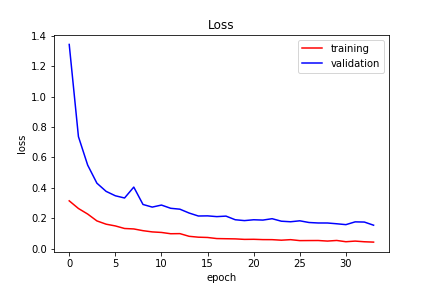
\includegraphics[width=\linewidth]{images/cae_online_lstm/caelstm_section_lstm_training_uniform_random_fill_10000_model_loss.png}
     \caption{Training/Validation Loss}
  \end{subfigure}
  \hfill
  \begin{subfigure}[b]{0.35\linewidth}
    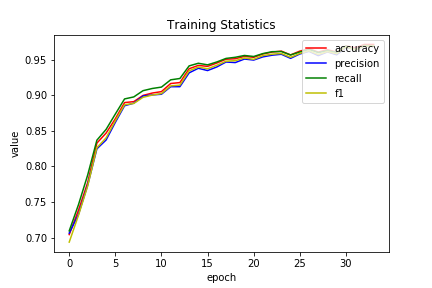
\includegraphics[width=\linewidth]{images/cae_online_lstm/caelstm_section_lstm_training_uniform_random_fill_10000_model_training_stats.png}
     \caption{Training Statistics}
  \end{subfigure}
  \hfill
  \begin{subfigure}[b]{0.35\linewidth}
    \includegraphics[width=\linewidth]{images/cae_online_lstm/caelstm_section_lstm_training_uniform_random_fill_10000_model_validation_stats.png}
     \caption{Validation Statistics}
  \end{subfigure}
  \caption{Training statistics for Algorithm \hyperref[tab: app_evalalgorithms]{6}}
  \label{fig: train_olnine_lstm_6}
\end{figure}

\begin{figure}[h!]
  \centerfloat
  \begin{subfigure}[b]{0.35\linewidth}
    \includegraphics[width=\linewidth]{images/cae_online_lstm/caelstm_section_lstm_training_block_map_10000_model_loss.png}
     \caption{Training/Validation Loss}
  \end{subfigure}
  \hfill
  \begin{subfigure}[b]{0.35\linewidth}
    \includegraphics[width=\linewidth]{images/cae_online_lstm/caelstm_section_lstm_training_block_map_10000_model_training_stats.png}
     \caption{Training Statistics}
  \end{subfigure}
  \hfill
  \begin{subfigure}[b]{0.35\linewidth}
    \includegraphics[width=\linewidth]{images/cae_online_lstm/caelstm_section_lstm_training_block_map_10000_model_validation_stats.png}
     \caption{Validation Statistics}
  \end{subfigure}
  \caption{Training statistics for Algorithm \hyperref[tab: app_evalalgorithms]{7}}
  \label{fig: train_olnine_lstm_7}
\end{figure}

\pagebreak

\begin{figure}[h!]
  \centerfloat
  \begin{subfigure}[b]{0.35\linewidth}
    \includegraphics[width=\linewidth]{images/cae_online_lstm/caelstm_section_lstm_training_house_10000_model_loss.png}
     \caption{Training/Validation Loss}
  \end{subfigure}
  \hfill
  \begin{subfigure}[b]{0.35\linewidth}
    \includegraphics[width=\linewidth]{images/cae_online_lstm/caelstm_section_lstm_training_house_10000_model_training_stats.png}
     \caption{Training Statistics}
  \end{subfigure}
  \hfill
  \begin{subfigure}[b]{0.35\linewidth}
    \includegraphics[width=\linewidth]{images/cae_online_lstm/caelstm_section_lstm_training_house_10000_model_validation_stats.png}
     \caption{Validation Statistics}
  \end{subfigure}
  \caption{Training statistics for Algorithm \hyperref[tab: app_evalalgorithms]{8}}
  \label{fig: train_olnine_lstm_8}
\end{figure}

\begin{figure}[h!]
  \centerfloat
  \begin{subfigure}[b]{0.35\linewidth}
    \includegraphics[width=\linewidth]{images/cae_online_lstm/caelstm_section_lstm_training_uniform_random_fill_10000_block_map_10000_model_loss.png}
     \caption{Training/Validation Loss}
  \end{subfigure}
  \hfill
  \begin{subfigure}[b]{0.35\linewidth}
    \includegraphics[width=\linewidth]{images/cae_online_lstm/caelstm_section_lstm_training_uniform_random_fill_10000_block_map_10000_model_training_stats.png}
     \caption{Training Statistics}
  \end{subfigure}
  \hfill
  \begin{subfigure}[b]{0.35\linewidth}
    \includegraphics[width=\linewidth]{images/cae_online_lstm/caelstm_section_lstm_training_uniform_random_fill_10000_block_map_10000_model_validation_stats.png}
     \caption{Validation Statistics}
  \end{subfigure}
  \caption{Training statistics for Algorithm \hyperref[tab: app_evalalgorithms]{9}}
  \label{fig: train_olnine_lstm_9}
\end{figure}

\begin{figure}[h!]
  \centerfloat
  \begin{subfigure}[b]{0.35\linewidth}
    \includegraphics[width=\linewidth]{images/cae_online_lstm/caelstm_section_lstm_training_uniform_random_fill_10000_block_map_10000_house_10000_model_loss.png}
     \caption{Training/Validation Loss}
  \end{subfigure}
  \hfill
  \begin{subfigure}[b]{0.35\linewidth}
    \includegraphics[width=\linewidth]{images/cae_online_lstm/caelstm_section_lstm_training_uniform_random_fill_10000_block_map_10000_house_10000_model_training_stats.png}
     \caption{Training Statistics}
  \end{subfigure}
  \hfill
  \begin{subfigure}[b]{0.35\linewidth}
    \includegraphics[width=\linewidth]{images/cae_online_lstm/caelstm_section_lstm_training_uniform_random_fill_10000_block_map_10000_house_10000_model_validation_stats.png}
     \caption{Validation Statistics}
  \end{subfigure}
  \caption{Training statistics for Algorithm \hyperref[tab: app_evalalgorithms]{10}}
  \label{fig: train_olnine_lstm_10}
\end{figure}

\pagebreak

\end{appendices}